

\chapter{Theory}
%{$\boldsymbol{ B_{s}^{0} \to \mu^{+} \mu^{-}}$}

% I should remember the Higgs, the Pentaquark and also graviational waves (when I talk about 4 fundemental forces).

Here is some text that I will happily explain, hmm the pdf does not update autmatically therefore this has not large benefit over using emails and compliting myself. What I really want is a text editing thing on my mac that lets me see the different colours.

Here I shall explain some theory stuff
The weak decays $B_{(s)}^{0} \to \mu^{+} \mu^{-}$ occur via flavour changing neutral currents (FCNC) in the Standard Model and are highly suppressed. 


$B_{s}^{0} \to \mu^{+} \mu^{-}$ was outlined as one of six important studies to be done at the LHCb \cite{RoadMap} due to the sensitivity of the branching fraction to contributions from new physics models.
Previously these rare decays have been studied at B factories and the Tevatron, and the current measurements for the branching fractions from the LHCb are 
$ \mathcal{B}(B_{s}^{0} \to \mu^{+} \mu^{-})  = (2.9_{-1.0}^{+1.1})\times 10^{-9}$ at 4.0 $\sigma$ significance and $ \mathcal{B}(B^{0} \to \mu^{+} \mu^{-}) < 7.4 \times 10^{-10}$ at $95\%$ CL.

In this section I shall introduce the Standard Model (Section 4.1) and outline how $B_{(s)}^{0} \to \mu^{+} \mu^{-}$ occurs within the Standard Model (Section 4.2). 
The calculation of the branching fractions for the decays is explained (Section 4.3) and finally, the current 
status for the search and measurements of  $B_{(s)}^{0} \to \mu^{+} \mu^{-}$ reviewed and future aims at the LHCb (Section 4.5).



\section{The Standard Model}

The Standard Model (SM) is a quantum field theory which describes matter and its interactions at a fundamental level. In the SM there are 12 fundamental spin-$\frac{1}{2}$ fermions; six quarks and six leptons. The six quarks form three families; up and down, strange and charm, top and bottom. Quarks have both electric and colour charge and combine into composite
particles either as a quark anti-quark pair to make a meson or as three quarks to make a baryon.\footnote{The Z(4430) is neither a meson or a baryon, it was first observed at Belle \cite{Choi:2007wga} and recently confirmed at the LHCb \cite{Aaij:2014jqa} with a 
high statistical significance. It is composed of four quarks and is the the first exotic particle to be observed at a high statistical significance.} Similarly leptons form three families each containing a charged and a neutral particle: $e^{-}$ 
and $\nu_{e}$, $\mu^{-}$ and $\nu_{\mu}$, $\tau^{-}$ and $\nu_{\tau}$, however leptons have no colour charge. 

Quarks and leptons interact through the strong force, weak force and electromagnetic force. The strong force is described by a symmetry group of $SU(3)_{C}$ colour charge, quarks
are the only coloured particles therefore the strong force acts only between quarks and anti-quarks. The strong force is mediated by 8 massless coloured gluons and its strength increases as distance between quarks increases. 

The electromagnetic force describes interactions between electrically charged particles. The gauge boson mediating the electromagnetic force is the photon, since the photon is massless the force
has in infinite range. 
The weak force allows interactions between all fermions in the SM, it allows flavour changing to occur between quarks or between charged leptons and their associated neutrinos. 
These interactions are mediated by massive gauge bosons; the $W^{\pm}$ and the $Z^{0}$. The weak and electromagnetic forces can be unified into a $SU(2) \otimes U(1)$ symmetry group. However 
is a broken symmetry because the gauge bosons have different masses for the two interactions. The Higgs mechanism accounts for this symmetry breaking, interactions of the electroweak bosons
with the Higgs field causes symmetry breaking creating the massive $W^{\pm}$ and $Z^{0}$ and the massless photon. 


The SM has evolved over time into what it is today, with discoveries prompting new theories and theoretical predictions motivation experimental searches. All fermions and bosons predicted in the SM have been discovered, the latest of these being the 
Higgs boson for which the ATLAS and CMS experiments discovered a possible candidate in 2013 \cite{Higgs_ATLAS, Higgs_CMS}. However there are several shortcomings of the SM and 
observed phenomena that it does not explain, a few examples are outlined below;
\begin{itemize}
 \item matter anti-matter asymmetry - as the universe was created matter and anti-matter would have been created in equal amounts, however the universe today is matter dominated. One process
that can cause this asymmetry is $CP$ violation, this effect enters the SM via the CKM matrix, however the effect is too small to account for the observed imbalance. 
 \item neutrinos have been observed to oscillate \cite{Fukuda:2001nk, Fukuda:1998fd, Davis_neutrinos}, in order for neutrinos to oscillate they must be massive particles but in the SM neutrinos are massless. However the SM can be adapted to include massive neutrinos without any fundamental changes.
 \item gravity is not explained by the SM
 \item astronomical observations have revealed that the rotational speed of galaxies does not match up with the speed expect from the amount of matter visible in the universe \cite{1973A&A,Zwicky:1933gu,1937ApJ}. 
If General Relativity is correct then there must be invisible matter which interacts via gravity to produce the extra mass. There is no candidate to explain this dark matter in the SM. 
\end{itemize}

Therefore despite the successes of the SM there must be New Physics beyond the SM that will explain its shortcomings.



\subsection{$\boldsymbol{ B_{(s)}^{0} \to \mu^{+} \mu^{-}}$ in the Standard Model }

$B_{s}^{0} \to \mu^{+} \mu^{-}$ and $B^{0} \to \mu^{+} \mu^{-}$ occur by flavour changing neutral currents (FCNC), they are highly suppressed decays in which quark flavour but not quark charge change. Flavour changes in quarks are allowed
in the SM via the CKM matrix. The CKM matrix relates mass and flavour quark eigenstates 

$$
 \begin{pmatrix}
  d' \\
  s' \\
  b'
 \end{pmatrix}
=
\begin{pmatrix}
  V_{ud} & V_{us} & V_{ub} \\
  V_{cd} & V_{cs} & V_{cb} \\
 V_{td} & V_{ts} & V_{tb} 
 \end{pmatrix}
 \begin{pmatrix}
  d \\
  s \\
  b
 \end{pmatrix}
$$
where the amplitude for an up quark to change flavour 
to a bottom quark is proportional to the CKM matrix element $|V_{ub}|^{2}$. The numerical magnitudes of the CKM matrix elements are given in Eq.~\eqref{eq:CKM_2} \cite{PDG}, it is clear that some flavour changes
are probably than other, e.g. a bottom quark will change into a top quark with a much greater amplitude than to any other quark.

\begin{equation} \label{eq:CKM_2}
V_{CKM} = 
\begin{pmatrix}
   0.97427\pm0.00015 & 0.22534\pm0.00065 & 0.00351^{0.00015}_{-0.00014} \\

    0.22520\pm0.00065 & 0.97344\pm0.00016 & 0.0412^{0.0011}_{-0.0005} \\


    0.00867^{+0.00029}_{−0.00031}  & 0.0404^{+0.0011}_{−0.0005} & 0.999146^{+0.000021}_{−0.000046}

 \end{pmatrix}
\end{equation}




All interactions in the CKM matrix are mediated by $W^{\pm}$, and are flavour and charge changing. The decays $B_{s}^{0} \to \mu^{+} \mu^{-}$ and $B^{0} \to \mu^{+} \mu^{-}$ do not 
change charge and therefore cannot occur at tree level. A $\mu^{+} \mu^{-}$ pair can be produced from a  $Z^{0}$, $\gamma$ or $H^{0}$ which the constituent quarks
of the $B^{0}$ and $B^{0}_{s}$ cannot create. Therefore these decays occur via loop diagram such as $Z^{0}$ penguins or box diagrams. Figure \ref{diagrams} shows the dominant
Feynman diagrams for $B_{s}^{0} \to \mu^{+} \mu^{-}$ and $B^{0} \to \mu^{+} \mu^{-}$. The intermediate quark in the loop diagrams is the top quark, contributions from other quarks 
are negligible due to very small coupling to the $b$ quark in the CKM matrix.


\begin{figure}
\begin{center}
\begin{minipage}[b]{0.9\linewidth}
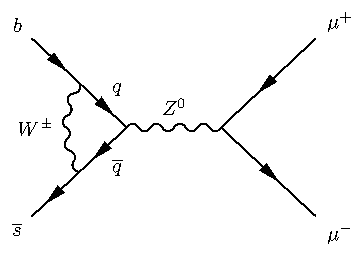
\includegraphics[width=0.4\linewidth]{df_bsmumu_SM_1.pdf}
\hspace{0.1\linewidth}
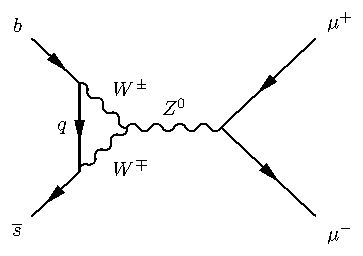
\includegraphics[width=0.4\linewidth]{df_bsmumu_SM_2.pdf}
\end{minipage}
\hspace{1cm}
\begin{minipage}[b]{0.9\linewidth}
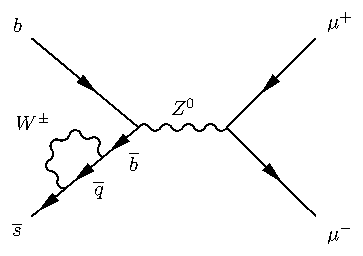
\includegraphics[width=0.4\linewidth]{df_bsmumu_SM_3.pdf}
\hspace{0.1\linewidth}
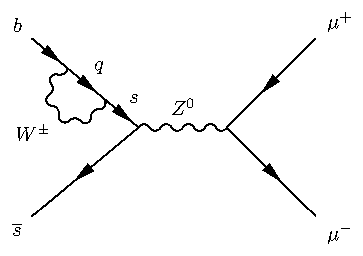
\includegraphics[width=0.4\linewidth]{df_bsmumu_SM_4.pdf}
\end{minipage}
\hspace{1cm}
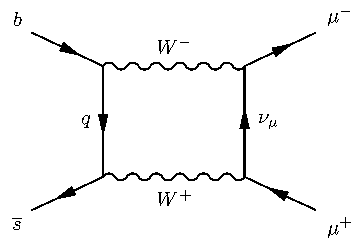
\includegraphics[width=0.36\linewidth]{df_bsmumu_SM_5.pdf}
\end{center}
\caption{Feynman diagrams dominant in the SM for $B_{s}^{0} \to \mu^{+} \mu^{-}$ \cite{Bettler:1257978}.}
\label{diagrams}

\end{figure}  
The decays $B_{s}^{0} \to \mu^{+} \mu^{-}$ and $B^{0} \to \mu^{+} \mu^{-}$ are not only suppressed because they are FCNC events they are also suppressed by a 
factor of

$$\left(\frac{m_{\mu}}{m_{B_{(s)}^{0}}}\right)^2$$
due to helicity. The $B$ hadron has zero spin therefore requiring the muons to have the same helicity.


%\begin{figure}
%\centering
%  \includegraphics[width = 0.85 \linewidth]{}
%  \caption{Feynman diagrams of leading order $B_{s}^{0} \to \mu^{+} \mu^{-}$, .}
%  \label{diagrams}
%\end{figure}



\section{Branching Fraction of $\boldsymbol{B_{(s)}^{0} \to \mu^{+} \mu^{-}}$ }

Weak decays such as $B_{(s)}^{0} \to \mu^{+} \mu^{-}$, can be described using a quantum field theory technique known at the Operator Product Expansion (OPE) \cite{Wilson:1969zs,Wilson:1972ee} to produce an effective Hamiltonian. The effective Hamiltonian 
divides the process into interactions on different distance scales and has the following form \cite{Buras:1998raa}

$$ H_{\textit{eff}} = \frac{G_{F}}{\sqrt{2}} \sum_{i} V^{i}_{CKM}\mathcal{C}(\mu)_{i} \mathcal{Q}(\mu)_{i} $$
%equation here from weak hamilt. ...
where $G_{F}$ is the Fermi constant, $\mathcal{C}(\mu)_i$ are Wilson coefficients and $\mathcal{Q}(\mu)_i$ are local operators.
The energy scale $\mu$ separates the interaction into two distance scales.  Wilson coefficients describe short scale processes, for energies greater than $\mu$, they incorporate contributions from internal loops and subsequently depend on $W^{\pm}$, $Z^{0}$,
$H^{0}$ and top quark masses. Perturbation theory can be used to calculate Wilson coefficients due to asymptotic freedom in QCD. The local operators $\mathcal{Q}_{i}$ describe long distance processes at energies smaller than $\mu$, they link initial and final decay states. 
These operators cannot be computed using perturbation theory and therefore have the greatest theoretical uncertainty in the in the Hamiltonian in many weak hadron decays.
The final Hamiltonian must be independent of $\mu$ because it is given an arbitrary size, often chosen as the mass of the decaying particle.

The effective Hamiltonian is a useful formalism for studying effects of new physics on weak decay because new physics contributions can enter the Hamiltonian though Wilson coefficients. 

For the decays $B_{s}^{0} \to \mu^{+} \mu^{-}$ and $B^{0} \to \mu^{+} \mu^{-}$ the effective Hamiltonian can be written as in \cite{Bobeth:2001sq}
\begin{equation} \label{eq:h_eff}
 H_{\textit{eff}} = -\frac{4G_{F}}{\sqrt{2} } V_{tb}V_{tq}^{*} \left [  \sum_{i=1}^{10}\mathcal{C}_{i} \mathcal{Q}_{i} + \mathcal{C}_{P} \mathcal{Q}_{P}+\mathcal{C}_{S} \mathcal{Q}_{S} + \mathcal{C}'_{P} \mathcal{Q}'_{P}+\mathcal{C}'_{S} \mathcal{Q}'_{S}\right ]
\end{equation} 
where $q$ corresponds to the other composite quark of $B$-hadron depending on whether is it $B^{0}$ or $B_{s}^{0}$ being considered in the Hamiltonian. The terms proportional to $ V_{tb}V_{uq}^{*}$ 
and  $V_{cb}V_{cq}^{*}$ are omitted from $H_{\textit{eff}}$ because their contribution is negligible compared to the CKM couplings to the top quark.

The only operators that have non-zero contributions in the decay amplitude for $B_{(s)}^{0} \to \mu^{+} \mu^{-}$ are

\begin{equation}
 \mathcal{Q}_{10} = \frac{e^{2}}{16 \pi^{2}}(\bar{q}\gamma^{\mu}P_{L}b)(\bar{l}\gamma_{\mu}\gamma_{5}l)
\end{equation}

\begin{equation}
 \mathcal{Q}_{S} = \frac{e^{2}}{16 \pi^{2}}m_{b}(\bar{q}P_{R}b)(\bar{l}l)
\end{equation}

\begin{equation}
 \mathcal{Q}_{P} =\frac{e^{2}}{16 \pi^{2}} m_{b}(\bar{q}P_{R}b)(\bar{l}\gamma_{5}l)
\end{equation}


\begin{equation}
 \mathcal{Q}'_{S} = \frac{e^{2}}{16 \pi^{2}}m_{q}(\bar{q}P_{L}b)(\bar{l}l)
\end{equation}

\begin{equation}
 \mathcal{Q}'_{P} =\frac{e^{2}}{16 \pi^{2}} m_{q}(\bar{q}P_{L}b)(\bar{l}\gamma_{5}l)
\end{equation}
%copied from analysis of neutral higgs
all other operators in equation \eqref{eq:h_eff} are zero due to the leptonic final states in $B_{(s)}^{0} \to \mu^{+} \mu^{-}$.

The dominant contribution in the SM Hamiltonian come from $\mathcal{C}_{10}$ which contains the contributions from $Z^{0}$ penguins and
$W$-box diagrams. Contributions from $\mathcal{C_{S}}$ and $\mathcal{C_{P}}$, corresponding to Higgs-penguins, are negligible in the SM and can be ignored. However these contributions can be substantially 
increased by new physics processes. The branching fraction can therefore be written as \cite{Bettler:1257978}

%\begin{equation}
 $$\mathcal{B}(B_{(s)}\to \mu^{+}\mu^{-}) = \frac{G_{F}^{2}\alpha^{2}}{16\pi^{3}\sin^{4}(\theta_{W})}|V_{tb}V_{tq}^{*}|^{2} \tau_{B_{(s)^{0}}}m_{B_{(s)^{0}}}f_{B_{(s)^{0}}}^{2}m_{\mu}^{2}\sqrt{1-\frac{4m_{\mu}^{2}}{m_{B_{(s)^{0}}}^{2}}}\mathcal{C}_{10}^{2}$$
where $f_{B_{(s)^{0}}}$ is the $B$-hadron decay factor, $\tau_{B_{(s)^{0}}}$ it's lifetime and $m_{B_{(s)^{0}}}$ it's mass.
The SM predictions for the branching fractions are \cite{Bobeth:2013uxa} 

$$ \mathcal{B}(B_{s}^{0} \to \mu^{+} \mu^{-}) = (3.65\pm0.23)\times 10^{-9}$$

$$ \mathcal{B}(B^{0} \to \mu^{+} \mu^{-}) = (1.06\pm0.09)\times 10^{-10}$$


The branching fraction  for $B^{0} \to \mu^{+} \mu^{-}$ is smaller than $B_{s}^{0} \to \mu^{+} \mu^{-}$ due to the CKM matrix contributions $\frac{|V_{tb}V_{td}^{*}|^{2}}{|V_{tb}V_{ts}^{*}|^{2}} \sim 0.044$ and larger helicity suppression, therefore although $B^{0}$ are produced in greater numbers at the LHC far fewer are observed. This has made the study of $B_{s}^{0} \to \mu^{+} \mu^{-}$ a greater priority at the LHCb.









